\documentclass[aspectratio=169,11pt]{beamer}
\usepackage[utf8]{inputenc}
\usepackage[T1]{fontenc}
\usepackage{lmodern,graphicx,amsmath,booktabs,array}
\usepackage{xcolor,tikz}
\usetikzlibrary{arrows.meta,positioning,calc,fit,shapes.geometric}

% Visual language retained from the supplied research-ideas template.
\definecolor{tumblue}{RGB}{0,101,189}
\definecolor{tumdark}{RGB}{0,51,89}
\definecolor{tumgray}{RGB}{105,105,105}
\definecolor{tumlight}{RGB}{235,243,248}
\definecolor{tumgreen}{RGB}{162,173,0}
\definecolor{tumorange}{RGB}{243,125,32}
\definecolor{tumred}{RGB}{229,52,24}
\definecolor{zeogray}{RGB}{218,213,202}
\definecolor{poreblue}{RGB}{94,181,226}
\definecolor{co2blue}{HTML}{2C7FB8}

\usetheme{default}
\setbeamertemplate{navigation symbols}{}
\setbeamercolor{normal text}{fg=black,bg=white}
\setbeamercolor{frametitle}{fg=tumblue}
\setbeamercolor{structure}{fg=tumblue}
\setbeamercolor{itemize item}{fg=tumblue}
\setbeamertemplate{itemize items}[circle]
\setbeamertemplate{headline}{%
  \leavevmode\begin{beamercolorbox}[wd=\paperwidth,ht=3.2ex,dp=1.6ex]{frametitle}
  \hfill\raisebox{-0.85cm}{
\includegraphics[height=0.8cm]{figures/tum_logo.png}}\hspace*{1em}
  \end{beamercolorbox}}
\setbeamertemplate{footline}{%
  \leavevmode\begin{beamercolorbox}[wd=\paperwidth,ht=3.2ex,dp=1.3ex]{author in head/foot}
  \hspace*{1em}\color{tumgray} Khalifa and Briesen \enspace|\enspace HeatPath--GNN
  \hfill\insertframenumber/\inserttotalframenumber\hspace*{1em}
  \end{beamercolorbox}}

\newcommand{\hi}[1]{\textcolor{tumblue}{\textbf{#1}}}
\newcommand{\question}[1]{\par%
  \begin{beamercolorbox}[rounded=true,sep=0.65em]{block body}
  \centering\large\color{tumdark}\textbf{#1}
  \end{beamercolorbox}}
\newcommand{\result}[1]{\par%
  \begin{beamercolorbox}[rounded=true,sep=0.55em]{block body}
  \centering\color{tumdark}\textbf{#1}
  \end{beamercolorbox}}
\newcommand{\source}[1]{\par\vfill{\tiny\color{tumgray}Source: #1}}
\tikzset{
  box/.style={draw=tumdark!75,rounded corners=2pt,fill=tumlight,
    align=center,minimum height=9mm,text width=2.55cm,font=\small,inner sep=3pt},
  arr/.style={-{Latex[length=2mm]},thick,tumblue},
  bead/.style={circle,draw=black!65,fill=zeogray,minimum size=6.4mm,inner sep=0pt},
  pore/.style={circle,draw=tumblue!80!black,fill=poreblue,minimum size=1.8mm,inner sep=0pt},
  throat/.style={draw=tumblue!82,line width=1.05pt}}

\newcommand{\FlexRowHeight}{}
\newenvironment{FlexRow}[1]{%
  \def\FlexRowHeight{#1}\begin{overlayarea}{\textwidth}{#1}\begin{columns}[T,onlytextwidth]
}{\end{columns}\end{overlayarea}}
\newcommand{\Col}[2]{\column{#1\textwidth}\begin{minipage}[t][\FlexRowHeight]{\linewidth}#2\end{minipage}}


\newcommand{\sectiondivider}[5]{%
\section[#3]{#3}
\begin{frame}{}
\centering
\vfill
{\color{tumgray}\large Section #1 of #2\par}
\vspace{.35cm}
{\color{tumblue}\LARGE\bfseries #3\par}
\vspace{.35cm}
{\large\color{tumdark}#4\par}
\vfill
\note{#5}
\end{frame}}

\setbeamertemplate{frametitle}{\vspace{0.05cm}\parbox{0.88\textwidth}{\large\color{tumblue}\insertframetitle}}
% \setbeameroption{show notes on second screen=right}
\begin{document}
\begin{frame}{}
\small
\begin{center}\Large\bfseries HeatPath--GNN\\[1ex]Learning where to place conductive particles\end{center}\vspace{.4cm}\begin{columns}[T,onlytextwidth]\column{.36\textwidth}\vspace{.4cm}\hi{Thermal transport through particle contact networks}\\[.6cm]Technical University of Munich\\Chair of Process Systems Engineering\\[.5cm]Ali Khalifa \& Heiko Briesen\column{.60\textwidth}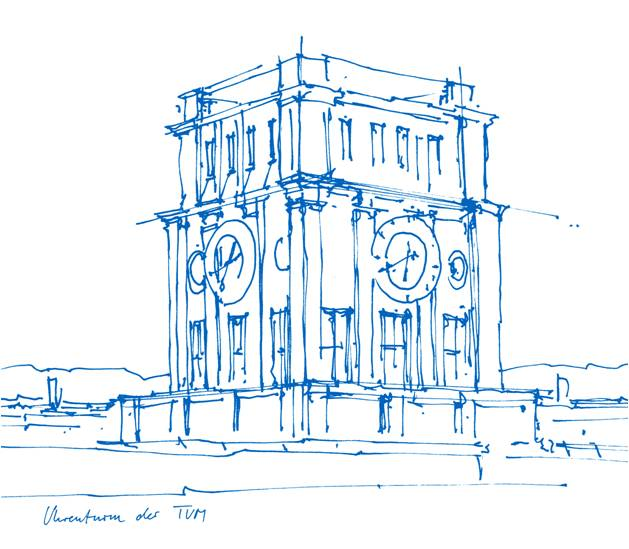
\includegraphics[width=\linewidth,height=4.1cm,keepaspectratio]{figures/uhrenturm.jpg}\end{columns}


\note{Today I will explain a particle-allocation problem. We have a fixed packed bed and a limited amount of highly conductive material. The question is where to place that material to improve heat transfer. We first solve and optimize a physical thermal network, then train a graph neural network to propose allocations for another packing. The results cover thirty independent realizations of one packing specification.}
\end{frame}
\begin{frame}{Outline}
\small
\tableofcontents[hideallsubsections]
\vspace{.35cm}
\result{The story moves from the physical allocation problem to fast prediction on an unseen packing.}
\note{The presentation follows five questions. Why does particle allocation matter? How do we convert the DEM packing into a thermal network? How do the reference methods and swap search generate strong allocations? What exactly does the GNN learn and predict? Finally, how much performance does it recover and at what computational cost?}
\end{frame}

\sectiondivider{1}{5}{Motivation and research question}{A fixed material budget turns heat transfer into an allocation problem}{This section defines the design problem. The packing and the amount of conductive material remain fixed. Only the particle material labels change.}

\begin{frame}{Motivation: conductive material is a limited resource}
\small
\begin{columns}[T,onlytextwidth]
\column{.55\textwidth}
\hi{Application examples}
\begin{itemize}
\item \textbf{Catalytic reactors:} conductive inert pellets spread heat but replace active catalyst.
\item \textbf{Adsorption beds:} graphite improves heat removal but replaces adsorbent.
\item \textbf{Thermal-storage beds:} conductive filler speeds charging but adds cost or replaces storage material.
\end{itemize}
\column{.41\textwidth}
\hi{Common design constraint}
\begin{itemize}
\item The conductive fraction is limited.
\item Packing geometry and size distribution remain fixed.
\item Particle placement becomes the design variable.
\end{itemize}
\end{columns}
\vspace{.25cm}
\result{Where should the limited conductive particles be placed to maximize heat conduction?}


\note{Several packed-bed applications contain a real material-budget trade-off. In catalytic reactors, conductive inert pellets such as silicon carbide can spread heat and reduce hot spots, but each inert pellet replaces active catalyst. Adsorption beds use graphite or other conductive additives to improve heat removal, but the additives reduce the amount of active sorbent. Thermal-storage beds can combine inexpensive storage material with a smaller conductive fraction, but that fraction adds cost or displaces storage capacity. These applications motivate the same design question studied here: if the conductive fraction, geometry and particle-size distribution are fixed, which particle positions should receive the conductive material? The present model isolates conduction through the solid contact network; it does not yet represent a complete reactor, adsorption unit or thermal-storage cycle.\par\medskip{\small Sources: Kulkarni et al. (2023), \textit{Catalysis Reviews}, doi:10.1080/01614940.2022.2025670; Fayazmanesh et al. (2017), \textit{Effective thermal conductivity modeling of consolidated sorption materials}; Ma et al. (2023), \textit{Numerical and experimental studies of packed-bed thermal energy storage}.}}
\end{frame}
\begin{frame}{The allocation problem}
\small
\centering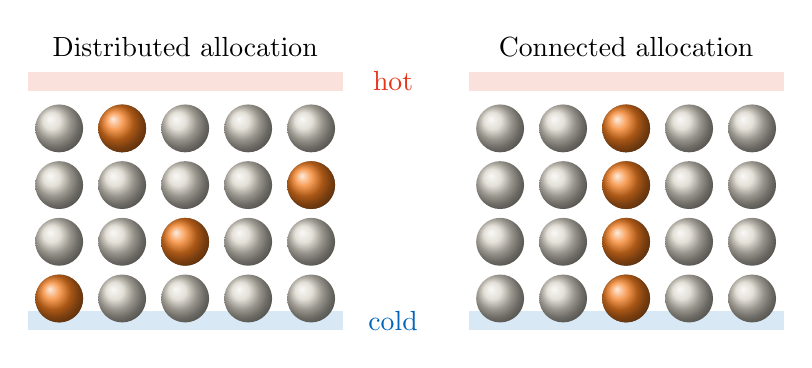
\begin{tikzpicture}[scale=.8]
\foreach \off/\lab in {0/Distributed allocation,7/Connected allocation}{
\fill[tumred!15] (\off-.5,3.3) rectangle (\off+4.5,3.6);
\fill[tumblue!15] (\off-.5,-.5) rectangle (\off+4.5,-.2);
\node at (\off+2,4) {\lab};
\foreach \x in {0,...,4}\foreach \y in {0,...,3}{\shade[ball color=zeogray] (\off+\x,\y*.9) circle (.38);}}
\foreach \x/\y in {0/0,2/1,4/2,1/3}{\shade[ball color=tumorange] (\x,\y*.9) circle (.38);}
\foreach \y in {0,...,3}{\shade[ball color=tumorange] (9,\y*.9) circle (.38);}
\node[tumred] at (5.3,3.45) {hot};\node[tumblue] at (5.3,-.35) {cold};
\end{tikzpicture}\par\small Orange: high conductivity. Grey: low conductivity. Schematic only.\par\vspace{.25cm}\result{Geometry and material amount stay fixed. Only particle labels change.}


\note{This schematic illustrates the hypothesis, not a measured packing or an optimal solution. Both arrangements contain the same number of orange particles. Connecting conductive particles could reduce resistance, but the whole network, including interfaces with low-conductivity particles, determines the result. The actual problem has five hundred particles and three size classes. We enforce the budget separately within each class, which also fixes the high-conductivity solid volume.}
\end{frame}
\sectiondivider{2}{5}{Packing and thermal model}{Particle contacts define the available heat-transfer routes}{This section explains how DEM contacts become a conservative thermal network. The thermal solver provides the particle temperatures, contact heat rates and whole-bed effective conductivity used throughout the study.}

\begin{frame}{Thirty packings with the same nominal porosity}
\small
\begin{columns}[T,onlytextwidth]\column{.48\textwidth}\begin{tabular}{lr}\toprule Quantity & Value\\\midrule Particles & 500\\Diameters [mm] & 1.5 / 2.0 / 2.5\\Counts & 100 / 300 / 100\\Nominal porosity & 0.38\\Independent seeds & 30\\\bottomrule\end{tabular}\column{.48\textwidth}\begin{itemize}\item Periodic boundaries in $x$ and $y$\item Two fixed thermal walls in $z$\item No gravity during generation\item Grow small spheres, then relax\item Accept final translational KE $\leq10^{-12}$ J\end{itemize}\end{columns}\vspace{.4cm}\small DEM: Hertz--Mindlin, $E=50$ MPa, $\nu=0.25$, restitution $0.30$, friction $0.50$.


\note{Each realization contains the same exact size distribution and occupies the same fixed-volume cell. Nominal porosity is calculated from the sum of sphere volumes divided by cell volume. With overlapping DEM spheres, this nominal quantity is not exactly the geometrical void fraction of their union. The modulus is deliberately softened. The final packings pass the particle-count, diameter, porosity, kinetic-energy and wall-spanning checks. We vary the random initialization, not the physical specification.}
\end{frame}
\begin{frame}{Contact conductance links temperature difference to heat rate}
\small
\begin{columns}[T,onlytextwidth]\column{.48\textwidth}\hi{Conductance: units W/K}
\[Q_{ij}=G_{ij}(T_i-T_j)\]
$G_{ij}$: between particles $i$ and $j$.\\[.15cm]
$G_{iw}$: between particle $i$ and wall $w$.\\[.15cm]
$Q_{ij}$: heat rate [W].\par\vspace{.2cm}
\small Material conductivity $k$ has units W/(m K).\column{.48\textwidth}\hi{Steady balance at particle $i$}
\[\sum_jG_{ij}(T_i-T_j)+\sum_wG_{iw}(T_i-T_w)=0\]
\hi{Whole-bed conductivity}
\[k_{\rm eff}=\frac{QH}{A(T_{\rm hot}-T_{\rm cold})}\]
$Q$: wall heat rate, $H$: height, $A$: wall area.\end{columns}\vspace{.3cm}\result{A larger conductance transfers more heat for the same temperature difference.}

\note{Here i and j identify particles, while w identifies a thermal wall. G is a conductance in watts per kelvin. Multiplying it by a temperature difference gives a heat rate in watts. For example, G equal to 0.01 W/K and a difference of 2 K gives 0.02 W. Material conductivity k has different units, W/(m K), because conductance also contains the contact geometry. Every internal contact contributes opposite heat rates to its two endpoints. The balance therefore conserves heat, and the net wall heat rate gives the effective bed conductivity. Fluid-gap conduction, radiation and convection are excluded.}
\end{frame}
\begin{frame}{Thermal conductance follows contact size and material}
\small
\begin{columns}[T,onlytextwidth]\column{.48\textwidth}\hi{Particle--particle contact}
\[a_{ij}=\sqrt{R_{ij}^{*}\delta_{ij}},\qquad R_{ij}^{*}=\frac{R_iR_j}{R_i+R_j}\]
\[G_{ij}=\frac{4a_{ij}k_i k_j}{k_i+k_j}\]
\small $\delta_{ij}$: geometric overlap.\\$a_{ij}$: Hertz contact radius.\column{.48\textwidth}\hi{Material assignment}
\[k_i\in\{1,10\}\;\mathrm{W\,m^{-1}K^{-1}}\]
\hi{Isothermal wall}
\[G_{iw}=4a_{iw}k_i\]
\small Two spreading resistances in series give the particle-contact formula.\end{columns}\vspace{.25cm}\small Ideal circular constriction model. Its small-contact assumption needs physical assessment.


\note{The contact radius comes from the Hertz geometrical relation between overlap and effective radius. The thermal model then adds two half-space spreading resistances, each equal to one over four k a. For identical conductivities this gives G equals two k a. An isothermal wall has zero spreading resistance on its side, leaving four k a. The corrected prefactor is used throughout this campaign. The formulas are idealizations, especially when the contact radius is not small compared with the particle radius.}
\end{frame}
\sectiondivider{3}{5}{Allocation methods and teacher search}{Boundary conditions, baseline solve, allocation methods and swap optimization}{This section follows the experiment in chronological order. We first impose the wall temperatures and fix the conductive-material quota. The all-low thermal solve supplies baseline temperatures and contact heat rates. We then compare allocation rules, improve the best reference with same-size swaps, and use the searched allocations as training targets.}

\begin{frame}{Thermal experiment and fixed material budget}
\small
\begin{columns}[T,onlytextwidth]
\column{.34\textwidth}
\hi{Boundary conditions}
\begin{itemize}
\item Bottom wall: $301$ K
\item Top wall: $300$ K
\item Periodic in $x$ and $y$
\item Steady contact conduction
\end{itemize}
\column{.62\textwidth}
\centering
\begin{tabular}{lrrr}\toprule Diameter [mm]&1.5&2.0&2.5\\\midrule Total particles&100&300&100\\High-$k$ particles&10&30&10\\\bottomrule\end{tabular}
\end{columns}
\vspace{.15cm}
\[\max_{\mathbf{s}}\; k_{\rm eff}(\mathbf{s}),\qquad s_i\in\{0,1\},\qquad\sum_{i\in\mathcal{B}_b}s_i=q_b\]
\small Here $s_i=1$ assigns high conductivity to particle $i$. The set $\mathcal B_b$ contains one size class, and $q_b$ fixes its number of high-$k$ particles. We change only the assignment $\mathbf s$ and seek the largest $k_{\rm eff}$.\par\vspace{.18cm}
\result{Fifty of 500 particles are conductive, with exactly 10\% in each size class.}


\note{We impose 301 K at the bottom wall and 300 K at the top wall. The lateral directions are periodic, and the present model includes steady conduction through particle contacts. The table fixes the conductive budget: ten, thirty and ten particles in the three size classes. The binary variable $s_i$ records the material assigned to particle $i$. A value of one means high conductivity. The set $\mathcal B_b$ contains the particles in size class $b$, and the equation fixes their sum to the quota $q_b$. The optimization changes only these material labels and seeks the allocation with the largest whole-bed effective conductivity.}
\end{frame}
\begin{frame}{All-low thermal solve before material allocation}
\small
\hi{Step 1: assign the low conductivity to every particle}
\[k_i=k_{\rm low}=1\;\mathrm{W\,m^{-1}K^{-1}}\qquad\text{for every particle}\]
\begin{columns}[T,onlytextwidth]\column{.48\textwidth}\hi{Baseline temperature $T_i^{(0)}$}
\par Solve the contact network between the 301 K bottom wall and the 300 K top wall. Each particle receives a baseline temperature.
\column{.48\textwidth}\hi{Baseline heat-throughput score}
\[s_i^{(0)}=\sum_{j\in\mathcal N(i)}\left|G_{ij}^{(0)}(T_i^{(0)}-T_j^{(0)})\right|\]
Sum the absolute heat rates at particle--particle contacts [W].
\end{columns}\vspace{.25cm}\result{The all-low solve supplies thermal features before any high-$k$ particles are selected.}

\note{This is the first thermal calculation for each packing. We assign the low conductivity to every particle, impose 301 K at the bottom wall and 300 K at the top wall, and solve the steady contact network. The solution gives a baseline temperature for each particle and a baseline heat rate for each contact. The heat-throughput score sums the absolute particle-contact heat rates incident on a particle. These baseline quantities are available before any high-conductivity particles are selected.}
\end{frame}
\begin{frame}{Reference methods select which 50 particles become conductive}
\small
\begin{tabular}{p{3.0cm}p{9.6cm}}\toprule Method & Selection rule within each size class\\\midrule
Random allocation & Draw 10 / 30 / 10 particles at random. Repeat 100 times and average the resulting bed conductivities.\\[.25cm]
Degree ranking & Count each particle's contacting neighbours. Select the 10 / 30 / 10 particles with the highest counts.\\[.25cm]
\shortstack[l]{Heat-throughput\\ranking} & First solve the all-low-conductivity bed. Select the 10 / 30 / 10 particles with the largest baseline heat-throughput scores.\\\bottomrule\end{tabular}
\vspace{.4cm}\result{Each allocation gives a list of high-conductivity particle IDs, then a thermal solve gives $k_{\rm eff}$.}

\note{All three methods produce particle selections, not temperature predictions. We assign high conductivity to the selected fifty particles and low conductivity to the remaining four hundred and fifty, then solve the thermal problem. The degree and heat-throughput rules give one allocation each. Random sampling gives one hundred allocations, and its reported conductivity is their mean. Quotas are applied separately within each size class. Heat-throughput ranking sorts the all-low thermal heat-throughput feature. It does not run a shortest-path algorithm.}
\end{frame}
\begin{frame}{Swap search starts from the better reference allocation}
\small
\begin{enumerate}
\item Evaluate the allocations from degree ranking and heat-throughput ranking.\par Start from whichever gives the larger $k_{\rm eff}$.
\item Randomly choose a size class, then one high-$k$ particle and one low-$k$ particle from that class.
\item Exchange their material labels and solve the thermal network.
\item Keep the swap if $k_{\rm eff}$ increases. Otherwise keep the previous allocation.
\end{enumerate}\vspace{.25cm}\result{Five runs use the same starting allocation and different random swap sequences.}
\small Each run proposes 3000 swaps. Retain the best final allocation found.

\note{The starting point is a complete fifty-particle selection. We compare the degree and heat-throughput selections and initialize every run with the better one; a tie favours degree. Each proposal samples a size class and then one selected and one unselected particle within it. Swapping their labels preserves the quota exactly. The code accepts an increase larger than a relative tolerance of 1e-12. All five runs have the same initial assignment but independent random proposal sequences. Their final selections supply the learning targets, and the best of their final conductivities supplies the search reference. This is not a proven global optimum.}
\end{frame}
\begin{frame}{Teacher allocations for model training}
\small
\centering
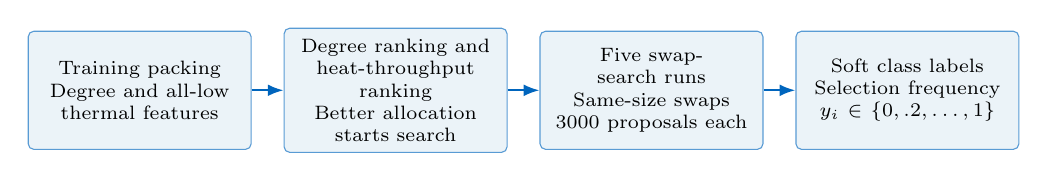
\begin{tikzpicture}[flow/.style={draw=tumblue!65,fill=tumlight,rounded corners=2pt,
text width=2.55cm,minimum height=1.5cm,align=center,font=\scriptsize,inner sep=4pt}]
\node[flow] (a) at (0,0) {Training packing\\Degree and all-low\\thermal features};
\node[flow] (b) at (3.25,0) {Degree ranking and\\heat-throughput ranking\\Better allocation starts search};
\node[flow] (c) at (6.5,0) {Five swap-search runs\\Same-size swaps\\3000 proposals each};
\node[flow] (d) at (9.75,0) {Soft class labels\\Selection frequency\\$y_i\in\{0,.2,\ldots,1\}$};
\draw[arr](a)--(b);\draw[arr](b)--(c);\draw[arr](c)--(d);
\end{tikzpicture}
\vspace{.45cm}
\begin{columns}[T,onlytextwidth]
\column{.48\textwidth}
\hi{Search output}\\
Each particle receives a target equal to the fraction of final search runs that selected it.
\column{.48\textwidth}
\hi{Scientific references}\\
Random, degree and heat-throughput allocations remain independent benchmarks for the learned models.
\end{columns}
\vspace{.3cm}
\result{The searched allocations provide training labels. They are not required when the trained GNN is applied.}
\note{This diagram now shows only model construction. For every training packing, we compute degree and the all-low thermal features. Degree ranking and heat-throughput ranking produce two valid allocations, and the better one initializes five independent swap-search runs. A particle's target is the fraction of the five final selections that contain it. Random, degree and heat-throughput remain separate benchmarks, but they are not required when the trained GNN is deployed.}
\end{frame}
\begin{frame}{Degree and heat throughput have three distinct roles}
\small
\begin{tabular}{>{\raggedright\arraybackslash}p{2.7cm}>{\raggedright\arraybackslash}p{5.3cm}>{\raggedright\arraybackslash}p{4.0cm}}\toprule Role & How the quantities are used & Output\\\midrule
1. Initialize search & Degree and heat-throughput rankings each select particles. & Better allocation starts swap search.\\[.3cm]
2. Supply features & GNN and MLP use both values during training and prediction. & Learned particle scores.\\[.3cm]
3. Compare methods & Evaluate both rankings on the held-out packing. & Reference $k_{\rm eff}$ values for comparison with GNN.\\\bottomrule\end{tabular}
\vspace{.4cm}\result{Feature: a value for each particle. Ranking method: a rule for selecting particles.}
\note{Degree is a neighbour count and heat throughput is a sum of absolute contact heat rates from the all-low thermal solve. Those are numerical features, available on both training and new packings. Degree ranking and heat-throughput ranking are allocation methods that sort those features within each size class and enforce the conductive-particle quotas. We use the resulting allocations to initialize the training-data search and as independent evaluation references. Using these features in a GNN does not force the GNN to reproduce either ranking: it can combine them with other particle information and contact messages. The MLP checks how much learning from the particle features achieves without those messages and edge features. For practical GNN prediction the features remain necessary, while running the reference allocation methods is optional benchmarking.}
\end{frame}
\sectiondivider{4}{5}{Graph learning and prediction}{The GNN learns a node-level classification score for material allocation}{This section explains the machine-learning task. The GNN performs node-level soft classification. It gives each particle a priority score, after which ranking within each size class enforces the exact material budget.}

\begin{frame}{The GNN uses geometry and the all-low thermal solution}
\small
\begin{columns}[T,onlytextwidth]\column{.48\textwidth}\hi{Eight particle features}\begin{itemize}\item Diameter, height and contact degree\item Hot-wall, cold-wall and anchored flags\item Normalized all-low temperature\item Normalized all-low heat-throughput score\end{itemize}\column{.48\textwidth}\hi{Six contact features}\begin{itemize}\item Contact radius\item Relative displacement in $x,y,z$\item Absolute vertical alignment\item Normalized absolute all-low contact heat rate\end{itemize}\end{columns}\vspace{.3cm}\small Three message-passing layers, width 64. MLP uses the same particle features. GNN additionally uses neighbour messages and contact features.

\note{The baseline quantities are normalized before entering the network. Anchored means connected through the thermal graph to an imposed-temperature boundary. Contact degree counts neighbouring particles, while the separate wall flags describe boundary contacts. The GNN passes information over the actual contact graph for three layers and uses the six edge features. The MLP sees the same eight node features but has no graph message passing or edge features. Consequently the comparison measures the benefit of this graph-based model and its contact information together. Dataset-wide feature standardization uses only the training packings.}
\end{frame}
\begin{frame}{The GNN performs particle classification}
\small
\centering
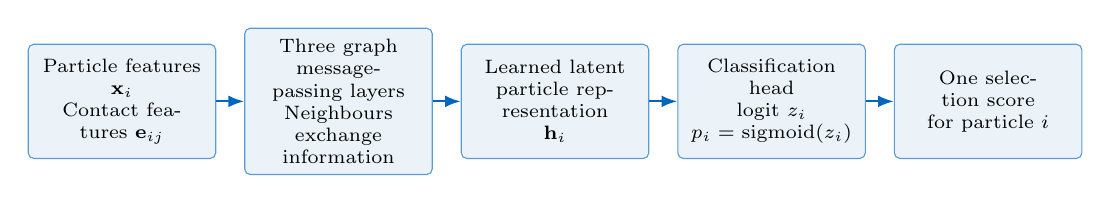
\begin{tikzpicture}[flow/.style={draw=tumblue!65,fill=tumlight,rounded corners=2pt,
text width=2.10cm,minimum height=1.45cm,align=center,font=\scriptsize,inner sep=4pt}]
\node[flow] (a) at (0,0) {Particle features\\$\mathbf{x}_i$\\Contact features $\mathbf{e}_{ij}$};
\node[flow] (b) at (2.75,0) {Three graph\\message-passing layers\\Neighbours exchange information};
\node[flow] (c) at (5.50,0) {Learned latent\\particle representation\\$\mathbf{h}_i$};
\node[flow] (d) at (8.25,0) {Classification head\\logit $z_i$\\$p_i=\mathrm{sigmoid}(z_i)$};
\node[flow] (e) at (11.00,0) {One selection score\\for particle $i$};
\draw[arr](a)--(b);\draw[arr](b)--(c);\draw[arr](c)--(d);\draw[arr](d)--(e);
\end{tikzpicture}
\vspace{.45cm}
\begin{columns}[T,onlytextwidth]
\column{.48\textwidth}
\hi{Training question}\\
How closely does this particle resemble particles retained by the teacher search?
\column{.48\textwidth}
\hi{Model output}\\
A continuous priority score for every particle, not the bed conductivity.
\end{columns}
\vspace{.3cm}
\result{This is node-level soft classification followed by constrained ranking.}
\note{The model performs node-level classification, not regression of effective conductivity. Each particle begins with eight node features, and every contact carries six edge features. Three message-passing layers combine the particle's own information with its neighbourhood and create a latent vector h for that particle. A small classification head converts h into a logit and sigmoid score. A high score means that the particle resembles particles repeatedly selected by the teacher search. The latent representation itself has no prescribed physical meaning.}
\end{frame}
\begin{frame}{Soft classification targets come from the search}
\small
\begin{columns}[T,onlytextwidth]
\column{.47\textwidth}
\hi{Target for particle $i$}
\[y_i=\frac{\text{final search runs selecting }i}{5}\]
Selection in four of five runs gives $y_i=0.8$.
\par\vspace{.25cm}
The target expresses search agreement, not a proven probability of global optimality.
\column{.49\textwidth}
\hi{Classification and ranking loss}
\[L=L_{\rm ranking}+0.2L_{\rm BCE}\]
BCE compares the sigmoid score $p_i$ with the soft label $y_i$.
\par\vspace{.2cm}
The ranking term favours particles with larger $y_i$ within the same size class.
\end{columns}
\vspace{.3cm}
\result{The network learns relative particle priorities. It does not regress $k_{\rm eff}$.}
\note{The target is soft because five searches may finish with different but similarly good allocations. If four of the five final allocations select particle i, its target is 0.8. Binary cross entropy trains the sigmoid output to agree with this selection frequency. The ranking term additionally preserves the relative order within a size class. The model therefore learns particle-selection priorities; it does not predict k effective.}
\end{frame}
\begin{frame}{Ranking within size classes enforces the budget}
\small
\begin{columns}[T,onlytextwidth]
\column{.48\textwidth}
\hi{The GNN scores all 500 particles}
\begin{itemize}
\item One continuous score per particle
\item Three trained repeats give three rankings
\item Average the ranks within each size class
\end{itemize}
\column{.48\textwidth}
\hi{Selection remains stratified}
\begin{itemize}
\item Top 10 among the 1.5 mm particles
\item Top 30 among the 2.0 mm particles
\item Top 10 among the 2.5 mm particles
\end{itemize}
\end{columns}
\vspace{.2cm}
\[
\mathcal S_b=\operatorname{Top}_{q_b}\{s_i:i\in\mathcal B_b\},
\qquad \mathcal S=\bigcup_b\mathcal S_b
\]
\vspace{.15cm}
\result{There is no global top-50 ranking across different particle sizes.}
\note{The GNN scores all five hundred particles, but we do not compare every score in one global list. We first separate the particles by diameter. Within each of the three size classes, each ensemble member supplies a ranking. We average those ranks and choose the top ten, thirty and ten particles. This avoids gaining an advantage merely by selecting more large particles and preserves the exact conductive-material volume.}
\end{frame}
\begin{frame}{Applying the trained GNN to a new packing}
\small
\centering
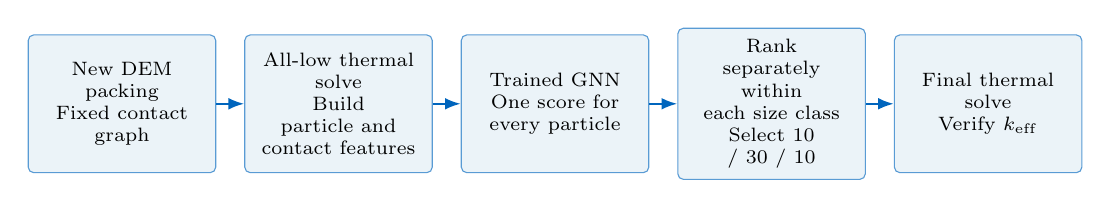
\begin{tikzpicture}[flow/.style={draw=tumblue!65,fill=tumlight,rounded corners=2pt,
text width=2.10cm,minimum height=1.75cm,align=center,font=\scriptsize,inner sep=4pt}]
\node[flow] (a) at (0,0) {\mbox{New} \mbox{DEM} \mbox{packing}\\\mbox{Fixed} \mbox{contact} \mbox{graph}};
\node[flow] (b) at (2.75,0) {\mbox{All-low} \mbox{thermal}\\\mbox{solve}\\\mbox{Build} \mbox{particle} \mbox{and}\\\mbox{contact} \mbox{features}};
\node[flow] (c) at (5.50,0) {\mbox{Trained} \mbox{GNN}\\\mbox{One} \mbox{score} \mbox{for}\\\mbox{every} \mbox{particle}};
\node[flow] (d) at (8.25,0) {\mbox{Rank}\\\mbox{separately} \mbox{within}\\\mbox{each} \mbox{size} \mbox{class}\\\mbox{Select} 10 / 30 / 10};
\node[flow] (e) at (11.00,0) {\mbox{Final} \mbox{thermal}\\\mbox{solve}\\\mbox{Verify} $k_{\rm eff}$};
\draw[arr](a)--(b);\draw[arr](b)--(c);\draw[arr](c)--(d);\draw[arr](d)--(e);
\end{tikzpicture}
\vspace{.45cm}
\begin{columns}[T,onlytextwidth]
\column{.48\textwidth}
\hi{Required for prediction}\\
One reference solve, feature construction, GNN scoring and quota selection.
\column{.48\textwidth}
\hi{Required only for evaluation}\\
Random, degree, heat-throughput and full swap-search comparisons.
\end{columns}
\vspace{.3cm}
\result{The trained GNN replaces the repeated swap search on the unseen packing.}
\note{For an unseen packing, we first solve the all-low-conductivity thermal network and construct the same node and edge features used during training. The trained GNN then scores every particle. Ranking is performed separately within each size class and selects ten, thirty and ten particles. One final thermal solve evaluates that proposed allocation. The swap search and the simple reference allocations are unnecessary for practical prediction; we run them on held-out cases only to evaluate the GNN.}
\end{frame}
\begin{frame}{Each test packing is withheld from model fitting}
\small
\centering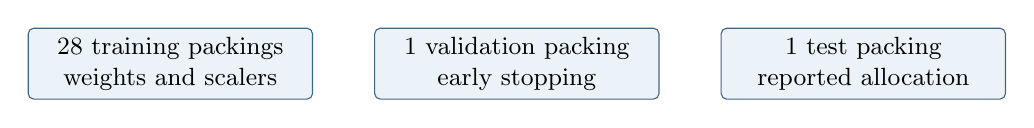
\begin{tikzpicture}
\node[box,text width=3.4cm] (a) at (0,0) {28 training packings\\weights and scalers};
\node[box,text width=3.4cm] (b) at (4.4,0) {1 validation packing\\early stopping};
\node[box,text width=3.4cm] (c) at (8.8,0) {1 test packing\\reported allocation};
\end{tikzpicture}\par\vspace{.5cm}\begin{itemize}\item Repeat for all 30 test packings\item Up to 400 epochs and patience 60\item Compare methods on the same held-out geometries\end{itemize}\vspace{.2cm}\result{This tests transfer between realizations of the specified packing.}


\note{The independent unit is the packing, not an individual particle. Splitting particles from the same bed between training and testing would expose almost the same structure on both sides. Here we hold out a whole packing, use another for validation and fit on the remaining twenty-eight. We repeat the process thirty times. These folds share training data, so they are not independent training experiments. This does not establish transfer to a new porosity, particle-size distribution, system size or material contrast.}
\end{frame}
\sectiondivider{5}{5}{Results and conclusions}{Graph information improves allocation with far fewer thermal solves}{This section compares all methods on complete held-out packings, reports conductivity gain and recovered search improvement, and closes with numerical limitations and future tests.}

\begin{frame}{Gain and recovery answer different questions}
\small
\[\mathrm{Gain}_m=100\frac{k_m-k_{\rm random}}{k_{\rm random}}\]
\[\mathrm{Recovery}_m=100\frac{k_m-k_{\rm random}}{k_{\rm search}-k_{\rm random}}\]
\vspace{.2cm}\begin{columns}[T,onlytextwidth]\column{.48\textwidth}\hi{Gain}\\How much better is this allocation than random?\column{.48\textwidth}\hi{Recovery}\\How much of the search improvement does the model obtain?\end{columns}\vspace{.4cm}\small Compute both per packing, then average. Error bars describe sample SD across packings.


\note{Gain normalizes the change by the random-allocation conductivity. Recovery instead divides by the available improvement found by the search. For example, a model that improves conductivity by thirty percent when search improves it by about fifty-two percent recovers roughly fifty-eight percent of the gain. The reported values are averages of per-packing ratios, so dividing displayed ensemble means will not necessarily reproduce them exactly. R-squared is not the performance measure for this discrete allocation task.}
\end{frame}
\begin{frame}{GNN improves conductivity by 30\% over random}
\small
\begin{columns}[T,onlytextwidth]\column{.60\textwidth}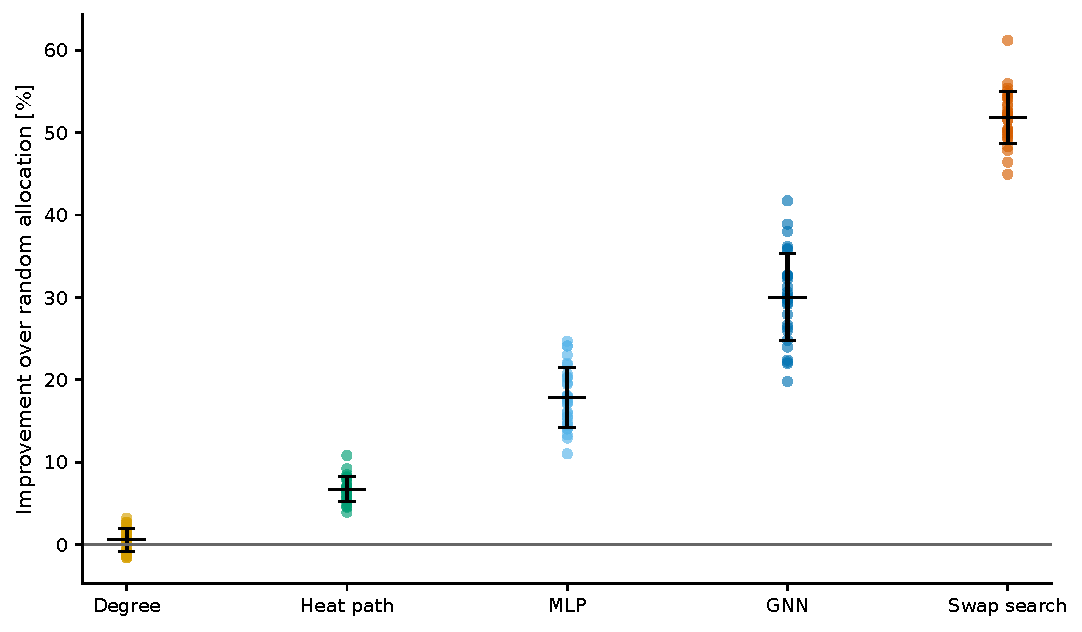
\includegraphics[width=\linewidth,height=.69\textheight,keepaspectratio]{figures/02_allocation_gain.pdf}\column{.36\textwidth}\hi{Mean improvement}\par\vspace{.2cm}\begin{tabular}{lr}Degree ranking&0.6\%\\\shortstack[l]{Heat-throughput\\ranking}&6.7\%\\MLP&17.9\%\\GNN&\textbf{30.0\%}\\Swap search&51.8\%\end{tabular}\vspace{.4cm}\par Same geometry and material budget for every comparison.\end{columns}


\note{The degree rule adds almost no average benefit. A homogeneous heat-throughput ranking is better, but both learned methods improve on it. The GNN delivers thirty percent mean gain relative to random assignment. Search still achieves substantially more, at fifty-one point eight percent. Each point is a packing, and the black summary marks show the mean and sample standard deviation. These results support learning useful allocation structure while also showing room for improvement.}
\end{frame}
\begin{frame}{Absolute conductivity remains below the search reference}
\small
\begin{columns}[T,onlytextwidth]\column{.60\textwidth}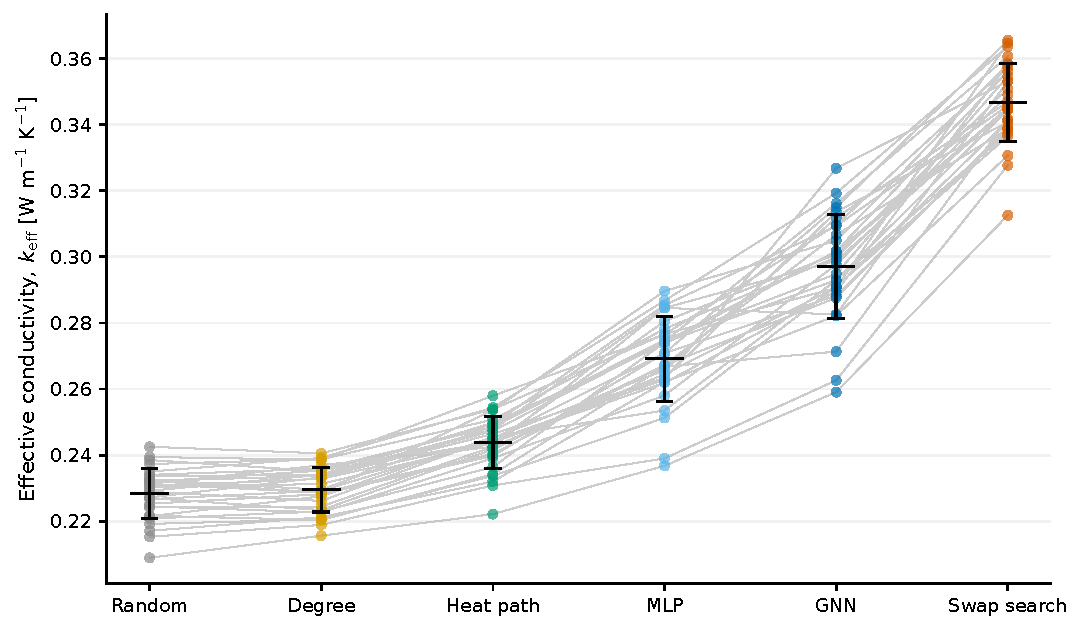
\includegraphics[width=\linewidth,height=.69\textheight,keepaspectratio]{figures/01_conductivity.pdf}\column{.36\textwidth}\hi{Mean $k_{\rm eff}$ [W/(m K)]}\par\vspace{.2cm}\begin{tabular}{lr}Random allocation&0.2284\\MLP&0.2692\\GNN&0.2970\\Swap search&0.3467\end{tabular}\vspace{.4cm}\par\small Grey lines connect results on the same packing.\end{columns}


\note{This slide gives the absolute scale of the conductivity changes. The mean rises from approximately 0.228 watts per metre kelvin for random assignment to 0.297 for the GNN. Search reaches approximately 0.347. The thin connecting lines preserve pairing across methods. These absolute numbers belong to the corrected contact-only model and should not be mixed with values from the earlier manuscript, which used a different thermal prefactor and packing-generation implementation.}
\end{frame}
\begin{frame}{GNN beats MLP on 29 of 30 held-out packings}
\small
\begin{columns}[T,onlytextwidth]\column{.60\textwidth}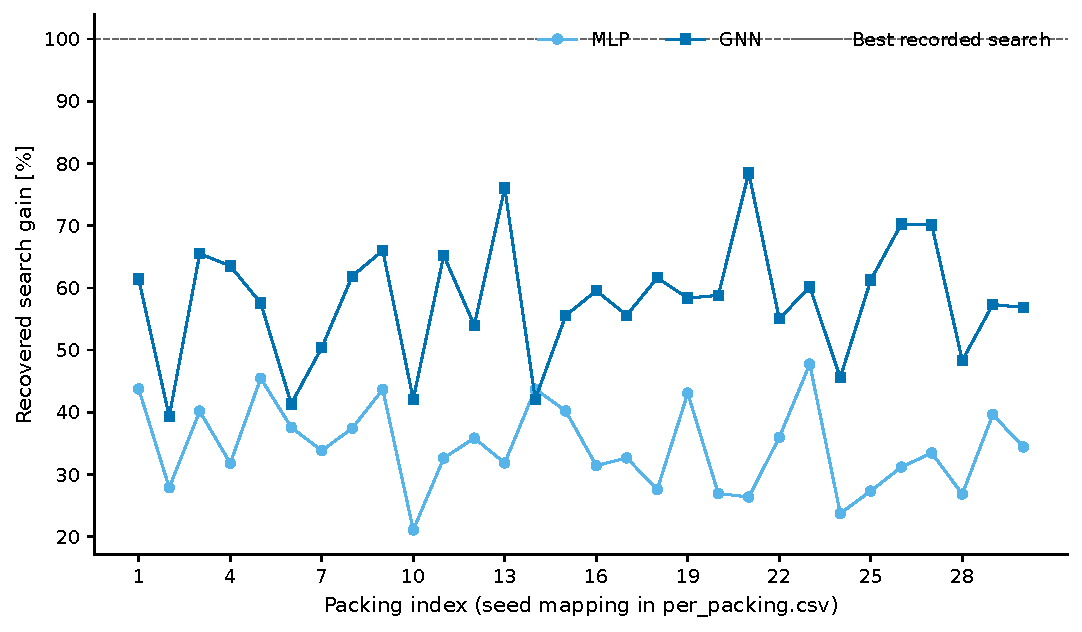
\includegraphics[width=\linewidth,height=.69\textheight,keepaspectratio]{figures/03_ml_recovery.pdf}\column{.36\textwidth}\hi{Recovered search improvement}\par\vspace{.2cm}GNN: \textbf{58.0\%}\\SD: 9.8 percentage points\\[.35cm]MLP: 34.5\% mean\\[.35cm]\small Improvement is consistent, but performance varies between packings.\end{columns}


\note{The GNN outperforms the MLP on twenty-nine of the thirty withheld packings. Its mean recovery is fifty-eight percent, with a standard deviation of nine point eight percentage points. This is descriptive evidence across our realizations, not a claim of independent folds or universal superiority. The gap to the search reference is still substantial. Both successful and less successful packings are included in this plot.}
\end{frame}
\begin{frame}{Contact-network diagnostics help interpret allocation}
\small
\begin{columns}[T,onlytextwidth]\column{.60\textwidth}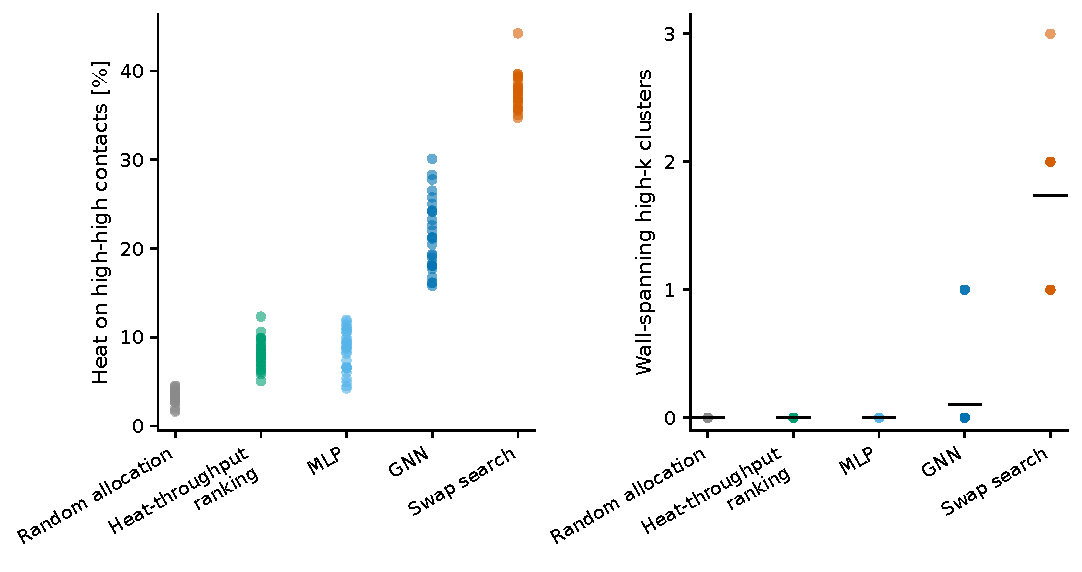
\includegraphics[width=\linewidth,height=.69\textheight,keepaspectratio]{figures/04_mechanisms.pdf}\column{.36\textwidth}\hi{Two diagnostics}\begin{itemize}\item Fraction of absolute contact heat carried by high--high contacts\item Number of high-conductivity clusters spanning both walls\end{itemize}\small These describe the selected network. They do not prove causality.\end{columns}


\note{The first diagnostic measures what fraction of summed absolute particle-contact heat rates occurs on contacts whose endpoints are both high-conductivity particles. This is not the fraction of net wall heat because heat can traverse multiple contacts. The second diagnostic asks whether the high-conductivity subgraph alone spans the two thermal boundaries. Low-conductivity particles can still participate in useful paths, so a spanning high-only cluster is not required for heat transfer. The random visualization uses the sampled assignment closest to the random mean.}
\end{frame}
\begin{frame}{Numerical checks pass, but contact sizes need scrutiny}
\small
\begin{columns}[T,onlytextwidth]\column{.60\textwidth}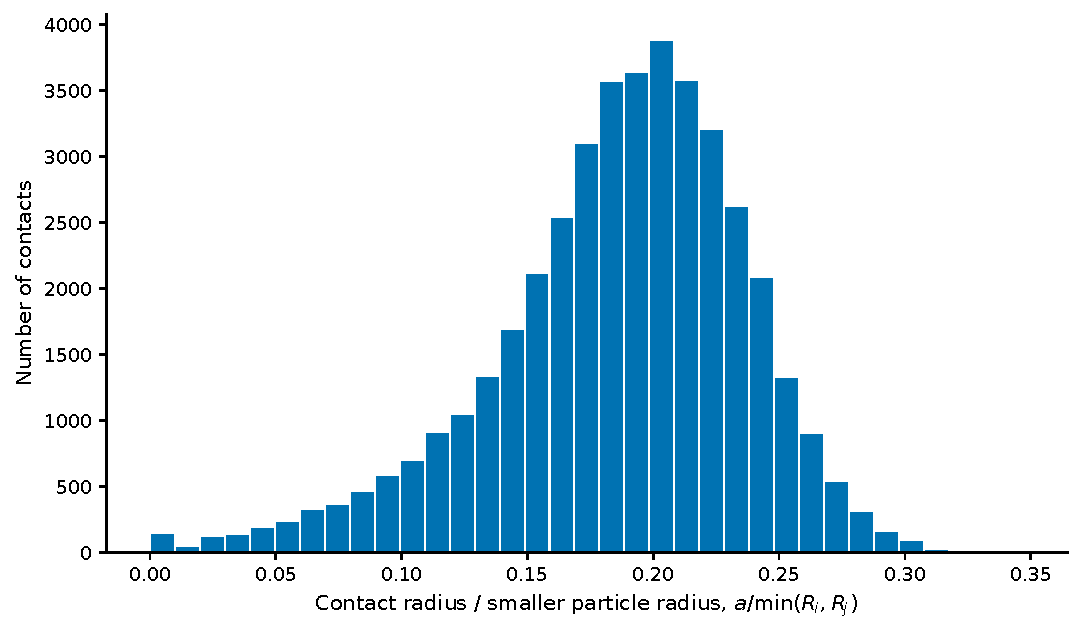
\includegraphics[width=\linewidth,height=.69\textheight,keepaspectratio]{figures/05_contact_geometry.pdf}\column{.36\textwidth}\hi{Recorded checks}\begin{itemize}\item Maximum final KE: $8.4\times10^{-13}$ J\item Maximum energy imbalance: $9.01\times10^{-12}$\end{itemize}\hi{Contact radius / smaller radius}\par Median: 0.192\\95th percentile: 0.258\\Maximum: 0.347\end{columns}


\note{The conservation and mechanical acceptance checks pass. However, numerical convergence does not establish physical validity. The contact-radius ratio has a median of about 0.19 and reaches about 0.35. Those contacts are not uniformly small relative to the particles. The half-space constriction approximation and the softened mechanical generation therefore deserve further assessment. This pooled histogram is a geometry diagnostic; individual contacts from the same bed are correlated.}
\end{frame}
\begin{frame}{The numerical overlap floor has little influence}
\small
\begin{columns}[T,onlytextwidth]\column{.60\textwidth}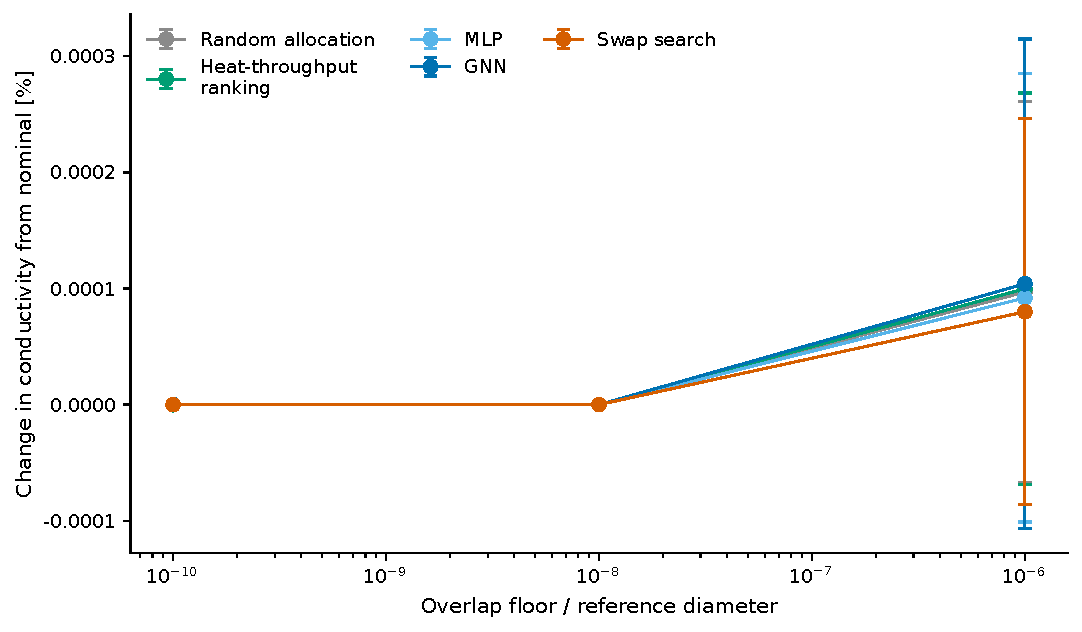
\includegraphics[width=\linewidth,height=.69\textheight,keepaspectratio]{figures/06_floor_sensitivity.pdf}\column{.36\textwidth}\hi{Fixed allocations}\begin{itemize}\item Vary the numerical overlap floor\item Largest absolute conductivity change: 0.000923\%\item Sensitivity is negligible over the tested range\end{itemize}\small This does not test stiffness, loading or alternative contact laws.\end{columns}


\note{A small overlap floor regularizes contact-radius evaluation. We repeat the thermal evaluation with different floor values while keeping the material assignments fixed. The largest absolute relative change is less than one thousandth of a percent. That is reassuring about this numerical choice. It does not resolve the physical contact-size concern on the previous slide, because we did not regenerate the beds under another modulus, pressure or contact model.}
\end{frame}
\begin{frame}{Fast scoring is one part of the complete prediction procedure}
\small
\begin{columns}[T,onlytextwidth]\column{.48\textwidth}\hi{What the reported times cover}\begin{itemize}\item Score all particles with trained models\item Mean GNN ensemble scoring: 8.63 ms\item Mean MLP ensemble scoring: 0.295 ms\end{itemize}\column{.48\textwidth}\hi{Additional work for a new packing}\begin{itemize}\item Solve the all-low-conductivity baseline\item Build particle and contact features\item Combine ranks and enforce quotas\item Solve the selected thermal network\end{itemize}\end{columns}\vspace{.3cm}\small Search uses about 14,964 thermal solves per packing. Training is an additional upfront cost.\par\vspace{.2cm}\result{Scoring time alone is insufficient to claim an end-to-end speedup.}

\note{Fast scoring means producing particle-priority scores with the already trained model. The quoted ensemble scoring time is the sum of forward-evaluation timings for the three model repeats. It excludes rank aggregation and exact quota selection as well as baseline solving, feature construction and final verification. Search uses nearly fifteen thousand candidate thermal solves per packing, which motivates replacing repeated search with learned priorities. However, this timing comparison is not a measurement of complete design time. Teacher-data generation and model training must also be considered when assessing amortized cost.}
\end{frame}
\begin{frame}{Conclusions and next research steps}
\small
\begin{columns}[T,onlytextwidth]\column{.48\textwidth}\hi{What the campaign establishes}\begin{itemize}\item Material placement strongly affects modelled conductivity\item GNN gains 30\% over random allocation\item Neighbour information improves on the MLP\item 58\% of best-found search gain is recovered\end{itemize}\column{.48\textwidth}\hi{What remains to establish}\begin{itemize}\item Physical sensitivity of contact areas\item Transfer to other packing specifications\item GNN-initialized search versus random starts\item Complete runtime and manufacturing feasibility\end{itemize}\end{columns}\vspace{.35cm}\result{A learned particle ranking captures useful thermal-network structure.}


\note{The main contribution is a constrained allocation workflow that combines a physical contact network with graph learning. Thirty independent packings give a clearer assessment than the earlier ten-case study. The results are promising, but the physical modelling assumptions and the remaining search-performance gap should shape the next work. A practical next algorithmic test is to initialize a short swap search with the GNN selection and compare its gain per thermal solve against random initialization. Physical sensitivity and external transfer should be evaluated before making broader claims.}
\end{frame}
\end{document}
